%        File: plotReport.tex
%     Created: Thu Sep 02 08:00 PM 2021 E
% Last Change: Thu Sep 02 08:00 PM 2021 E
%
\documentclass[a4paper]{article}
\usepackage{gnuplot-lua-tikz}
\usepackage{pgfplots}
\usepackage{mathtools}
\begin{document}

The goal of this script is to create a function with several kinks (and anti -
kinks

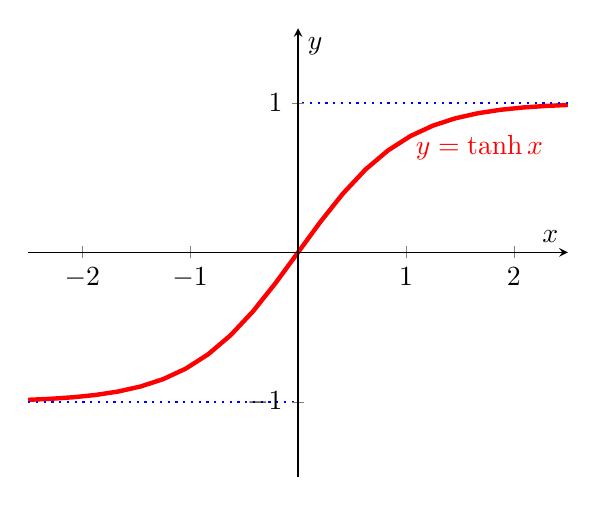
\begin{tikzpicture}
\begin{axis}[
    xmin=-2.5, xmax=2.5,
    ymin=-1.5, ymax=1.5,
    axis lines=center,
    axis on top=true,
    domain=-2.5:2.5,
    ylabel=$y$,
    xlabel=$x$,
    ]

    \addplot [mark=none,draw=red,ultra thick] {tanh(\x)};
    \node [right, red] at (axis cs: 1,0.7) {$y = \tanh x$};
    
    %% Add the asymptotes
    \draw [blue, dotted, thick] (axis cs:-2.5,-1)-- (axis cs:0,-1);
    \draw [blue, dotted, thick] (axis cs:+2.5,+1)-- (axis cs:0,+1);
\end{axis}
\end{tikzpicture}

\begin{align*}
    y = \tanh \left( x - 1 \right)
\end{align*}
\begin{figure}
    \begin{center}
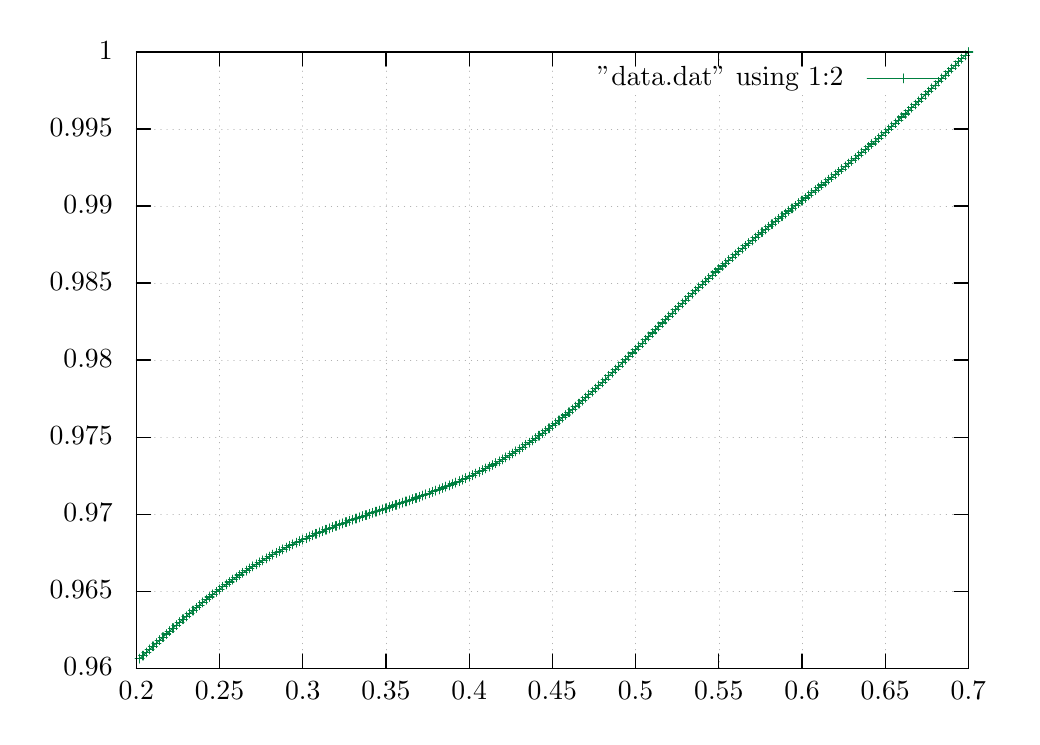
\begin{tikzpicture}[gnuplot]
%% generated with GNUPLOT 5.2p8 (Lua 5.3; terminal rev. Nov 2018, script rev. 108)
%% Fri 10 Sep 2021 09:17:21 AM EDT
\path (0.000,0.000) rectangle (12.500,8.750);
\gpcolor{color=gp lt color axes}
\gpsetlinetype{gp lt axes}
\gpsetdashtype{gp dt axes}
\gpsetlinewidth{0.50}
\draw[gp path] (1.380,0.616)--(11.947,0.616);
\gpcolor{color=gp lt color border}
\gpsetlinetype{gp lt border}
\gpsetdashtype{gp dt solid}
\gpsetlinewidth{1.00}
\draw[gp path] (1.380,0.616)--(1.560,0.616);
\draw[gp path] (11.947,0.616)--(11.767,0.616);
\node[gp node right] at (1.196,0.616) {$0.96$};
\gpcolor{color=gp lt color axes}
\gpsetlinetype{gp lt axes}
\gpsetdashtype{gp dt axes}
\gpsetlinewidth{0.50}
\draw[gp path] (1.380,1.594)--(11.947,1.594);
\gpcolor{color=gp lt color border}
\gpsetlinetype{gp lt border}
\gpsetdashtype{gp dt solid}
\gpsetlinewidth{1.00}
\draw[gp path] (1.380,1.594)--(1.560,1.594);
\draw[gp path] (11.947,1.594)--(11.767,1.594);
\node[gp node right] at (1.196,1.594) {$0.965$};
\gpcolor{color=gp lt color axes}
\gpsetlinetype{gp lt axes}
\gpsetdashtype{gp dt axes}
\gpsetlinewidth{0.50}
\draw[gp path] (1.380,2.572)--(11.947,2.572);
\gpcolor{color=gp lt color border}
\gpsetlinetype{gp lt border}
\gpsetdashtype{gp dt solid}
\gpsetlinewidth{1.00}
\draw[gp path] (1.380,2.572)--(1.560,2.572);
\draw[gp path] (11.947,2.572)--(11.767,2.572);
\node[gp node right] at (1.196,2.572) {$0.97$};
\gpcolor{color=gp lt color axes}
\gpsetlinetype{gp lt axes}
\gpsetdashtype{gp dt axes}
\gpsetlinewidth{0.50}
\draw[gp path] (1.380,3.550)--(11.947,3.550);
\gpcolor{color=gp lt color border}
\gpsetlinetype{gp lt border}
\gpsetdashtype{gp dt solid}
\gpsetlinewidth{1.00}
\draw[gp path] (1.380,3.550)--(1.560,3.550);
\draw[gp path] (11.947,3.550)--(11.767,3.550);
\node[gp node right] at (1.196,3.550) {$0.975$};
\gpcolor{color=gp lt color axes}
\gpsetlinetype{gp lt axes}
\gpsetdashtype{gp dt axes}
\gpsetlinewidth{0.50}
\draw[gp path] (1.380,4.529)--(11.947,4.529);
\gpcolor{color=gp lt color border}
\gpsetlinetype{gp lt border}
\gpsetdashtype{gp dt solid}
\gpsetlinewidth{1.00}
\draw[gp path] (1.380,4.529)--(1.560,4.529);
\draw[gp path] (11.947,4.529)--(11.767,4.529);
\node[gp node right] at (1.196,4.529) {$0.98$};
\gpcolor{color=gp lt color axes}
\gpsetlinetype{gp lt axes}
\gpsetdashtype{gp dt axes}
\gpsetlinewidth{0.50}
\draw[gp path] (1.380,5.507)--(11.947,5.507);
\gpcolor{color=gp lt color border}
\gpsetlinetype{gp lt border}
\gpsetdashtype{gp dt solid}
\gpsetlinewidth{1.00}
\draw[gp path] (1.380,5.507)--(1.560,5.507);
\draw[gp path] (11.947,5.507)--(11.767,5.507);
\node[gp node right] at (1.196,5.507) {$0.985$};
\gpcolor{color=gp lt color axes}
\gpsetlinetype{gp lt axes}
\gpsetdashtype{gp dt axes}
\gpsetlinewidth{0.50}
\draw[gp path] (1.380,6.485)--(11.947,6.485);
\gpcolor{color=gp lt color border}
\gpsetlinetype{gp lt border}
\gpsetdashtype{gp dt solid}
\gpsetlinewidth{1.00}
\draw[gp path] (1.380,6.485)--(1.560,6.485);
\draw[gp path] (11.947,6.485)--(11.767,6.485);
\node[gp node right] at (1.196,6.485) {$0.99$};
\gpcolor{color=gp lt color axes}
\gpsetlinetype{gp lt axes}
\gpsetdashtype{gp dt axes}
\gpsetlinewidth{0.50}
\draw[gp path] (1.380,7.463)--(11.947,7.463);
\gpcolor{color=gp lt color border}
\gpsetlinetype{gp lt border}
\gpsetdashtype{gp dt solid}
\gpsetlinewidth{1.00}
\draw[gp path] (1.380,7.463)--(1.560,7.463);
\draw[gp path] (11.947,7.463)--(11.767,7.463);
\node[gp node right] at (1.196,7.463) {$0.995$};
\gpcolor{color=gp lt color axes}
\gpsetlinetype{gp lt axes}
\gpsetdashtype{gp dt axes}
\gpsetlinewidth{0.50}
\draw[gp path] (1.380,8.441)--(11.947,8.441);
\gpcolor{color=gp lt color border}
\gpsetlinetype{gp lt border}
\gpsetdashtype{gp dt solid}
\gpsetlinewidth{1.00}
\draw[gp path] (1.380,8.441)--(1.560,8.441);
\draw[gp path] (11.947,8.441)--(11.767,8.441);
\node[gp node right] at (1.196,8.441) {$1$};
\gpcolor{color=gp lt color axes}
\gpsetlinetype{gp lt axes}
\gpsetdashtype{gp dt axes}
\gpsetlinewidth{0.50}
\draw[gp path] (1.380,0.616)--(1.380,8.441);
\gpcolor{color=gp lt color border}
\gpsetlinetype{gp lt border}
\gpsetdashtype{gp dt solid}
\gpsetlinewidth{1.00}
\draw[gp path] (1.380,0.616)--(1.380,0.796);
\draw[gp path] (1.380,8.441)--(1.380,8.261);
\node[gp node center] at (1.380,0.308) {$0.2$};
\gpcolor{color=gp lt color axes}
\gpsetlinetype{gp lt axes}
\gpsetdashtype{gp dt axes}
\gpsetlinewidth{0.50}
\draw[gp path] (2.437,0.616)--(2.437,8.441);
\gpcolor{color=gp lt color border}
\gpsetlinetype{gp lt border}
\gpsetdashtype{gp dt solid}
\gpsetlinewidth{1.00}
\draw[gp path] (2.437,0.616)--(2.437,0.796);
\draw[gp path] (2.437,8.441)--(2.437,8.261);
\node[gp node center] at (2.437,0.308) {$0.25$};
\gpcolor{color=gp lt color axes}
\gpsetlinetype{gp lt axes}
\gpsetdashtype{gp dt axes}
\gpsetlinewidth{0.50}
\draw[gp path] (3.493,0.616)--(3.493,8.441);
\gpcolor{color=gp lt color border}
\gpsetlinetype{gp lt border}
\gpsetdashtype{gp dt solid}
\gpsetlinewidth{1.00}
\draw[gp path] (3.493,0.616)--(3.493,0.796);
\draw[gp path] (3.493,8.441)--(3.493,8.261);
\node[gp node center] at (3.493,0.308) {$0.3$};
\gpcolor{color=gp lt color axes}
\gpsetlinetype{gp lt axes}
\gpsetdashtype{gp dt axes}
\gpsetlinewidth{0.50}
\draw[gp path] (4.550,0.616)--(4.550,8.441);
\gpcolor{color=gp lt color border}
\gpsetlinetype{gp lt border}
\gpsetdashtype{gp dt solid}
\gpsetlinewidth{1.00}
\draw[gp path] (4.550,0.616)--(4.550,0.796);
\draw[gp path] (4.550,8.441)--(4.550,8.261);
\node[gp node center] at (4.550,0.308) {$0.35$};
\gpcolor{color=gp lt color axes}
\gpsetlinetype{gp lt axes}
\gpsetdashtype{gp dt axes}
\gpsetlinewidth{0.50}
\draw[gp path] (5.607,0.616)--(5.607,8.441);
\gpcolor{color=gp lt color border}
\gpsetlinetype{gp lt border}
\gpsetdashtype{gp dt solid}
\gpsetlinewidth{1.00}
\draw[gp path] (5.607,0.616)--(5.607,0.796);
\draw[gp path] (5.607,8.441)--(5.607,8.261);
\node[gp node center] at (5.607,0.308) {$0.4$};
\gpcolor{color=gp lt color axes}
\gpsetlinetype{gp lt axes}
\gpsetdashtype{gp dt axes}
\gpsetlinewidth{0.50}
\draw[gp path] (6.663,0.616)--(6.663,8.441);
\gpcolor{color=gp lt color border}
\gpsetlinetype{gp lt border}
\gpsetdashtype{gp dt solid}
\gpsetlinewidth{1.00}
\draw[gp path] (6.663,0.616)--(6.663,0.796);
\draw[gp path] (6.663,8.441)--(6.663,8.261);
\node[gp node center] at (6.663,0.308) {$0.45$};
\gpcolor{color=gp lt color axes}
\gpsetlinetype{gp lt axes}
\gpsetdashtype{gp dt axes}
\gpsetlinewidth{0.50}
\draw[gp path] (7.720,0.616)--(7.720,7.953);
\draw[gp path] (7.720,8.261)--(7.720,8.441);
\gpcolor{color=gp lt color border}
\gpsetlinetype{gp lt border}
\gpsetdashtype{gp dt solid}
\gpsetlinewidth{1.00}
\draw[gp path] (7.720,0.616)--(7.720,0.796);
\draw[gp path] (7.720,8.441)--(7.720,8.261);
\node[gp node center] at (7.720,0.308) {$0.5$};
\gpcolor{color=gp lt color axes}
\gpsetlinetype{gp lt axes}
\gpsetdashtype{gp dt axes}
\gpsetlinewidth{0.50}
\draw[gp path] (8.777,0.616)--(8.777,7.953);
\draw[gp path] (8.777,8.261)--(8.777,8.441);
\gpcolor{color=gp lt color border}
\gpsetlinetype{gp lt border}
\gpsetdashtype{gp dt solid}
\gpsetlinewidth{1.00}
\draw[gp path] (8.777,0.616)--(8.777,0.796);
\draw[gp path] (8.777,8.441)--(8.777,8.261);
\node[gp node center] at (8.777,0.308) {$0.55$};
\gpcolor{color=gp lt color axes}
\gpsetlinetype{gp lt axes}
\gpsetdashtype{gp dt axes}
\gpsetlinewidth{0.50}
\draw[gp path] (9.834,0.616)--(9.834,7.953);
\draw[gp path] (9.834,8.261)--(9.834,8.441);
\gpcolor{color=gp lt color border}
\gpsetlinetype{gp lt border}
\gpsetdashtype{gp dt solid}
\gpsetlinewidth{1.00}
\draw[gp path] (9.834,0.616)--(9.834,0.796);
\draw[gp path] (9.834,8.441)--(9.834,8.261);
\node[gp node center] at (9.834,0.308) {$0.6$};
\gpcolor{color=gp lt color axes}
\gpsetlinetype{gp lt axes}
\gpsetdashtype{gp dt axes}
\gpsetlinewidth{0.50}
\draw[gp path] (10.890,0.616)--(10.890,7.953);
\draw[gp path] (10.890,8.261)--(10.890,8.441);
\gpcolor{color=gp lt color border}
\gpsetlinetype{gp lt border}
\gpsetdashtype{gp dt solid}
\gpsetlinewidth{1.00}
\draw[gp path] (10.890,0.616)--(10.890,0.796);
\draw[gp path] (10.890,8.441)--(10.890,8.261);
\node[gp node center] at (10.890,0.308) {$0.65$};
\gpcolor{color=gp lt color axes}
\gpsetlinetype{gp lt axes}
\gpsetdashtype{gp dt axes}
\gpsetlinewidth{0.50}
\draw[gp path] (11.947,0.616)--(11.947,8.441);
\gpcolor{color=gp lt color border}
\gpsetlinetype{gp lt border}
\gpsetdashtype{gp dt solid}
\gpsetlinewidth{1.00}
\draw[gp path] (11.947,0.616)--(11.947,0.796);
\draw[gp path] (11.947,8.441)--(11.947,8.261);
\node[gp node center] at (11.947,0.308) {$0.7$};
\draw[gp path] (1.380,8.441)--(1.380,0.616)--(11.947,0.616)--(11.947,8.441)--cycle;
\node[gp node right] at (10.479,8.107) {"data.dat" using 1:2};
\gpcolor{rgb color={0.000,0.502,0.251}}
\draw[gp path] (10.663,8.107)--(11.579,8.107);
\draw[gp path] (1.422,0.736)--(1.465,0.775)--(1.507,0.815)--(1.549,0.854)--(1.591,0.894)%
  --(1.634,0.933)--(1.676,0.972)--(1.718,1.010)--(1.760,1.049)--(1.803,1.087)--(1.845,1.125)%
  --(1.887,1.163)--(1.929,1.201)--(1.972,1.238)--(2.014,1.274)--(2.056,1.311)--(2.099,1.347)%
  --(2.141,1.382)--(2.183,1.417)--(2.225,1.452)--(2.268,1.486)--(2.310,1.519)--(2.352,1.553)%
  --(2.394,1.585)--(2.437,1.617)--(2.479,1.649)--(2.521,1.680)--(2.564,1.710)--(2.606,1.740)%
  --(2.648,1.770)--(2.690,1.799)--(2.733,1.827)--(2.775,1.855)--(2.817,1.882)--(2.859,1.908)%
  --(2.902,1.935)--(2.944,1.960)--(2.986,1.985)--(3.028,2.010)--(3.071,2.034)--(3.113,2.057)%
  --(3.155,2.080)--(3.198,2.103)--(3.240,2.125)--(3.282,2.147)--(3.324,2.168)--(3.367,2.189)%
  --(3.409,2.209)--(3.451,2.229)--(3.493,2.248)--(3.536,2.267)--(3.578,2.286)--(3.620,2.304)%
  --(3.662,2.322)--(3.705,2.340)--(3.747,2.357)--(3.789,2.374)--(3.832,2.391)--(3.874,2.407)%
  --(3.916,2.423)--(3.958,2.439)--(4.001,2.455)--(4.043,2.471)--(4.085,2.486)--(4.127,2.501)%
  --(4.170,2.516)--(4.212,2.531)--(4.254,2.546)--(4.296,2.560)--(4.339,2.575)--(4.381,2.589)%
  --(4.423,2.603)--(4.466,2.618)--(4.508,2.632)--(4.550,2.646)--(4.592,2.661)--(4.635,2.675)%
  --(4.677,2.689)--(4.719,2.704)--(4.761,2.718)--(4.804,2.733)--(4.846,2.747)--(4.888,2.762)%
  --(4.931,2.777)--(4.973,2.792)--(5.015,2.808)--(5.057,2.823)--(5.100,2.839)--(5.142,2.855)%
  --(5.184,2.871)--(5.226,2.887)--(5.269,2.904)--(5.311,2.921)--(5.353,2.938)--(5.395,2.955)%
  --(5.438,2.973)--(5.480,2.992)--(5.522,3.010)--(5.565,3.029)--(5.607,3.048)--(5.649,3.068)%
  --(5.691,3.088)--(5.734,3.109)--(5.776,3.130)--(5.818,3.152)--(5.860,3.174)--(5.903,3.196)%
  --(5.945,3.219)--(5.987,3.243)--(6.029,3.267)--(6.072,3.292)--(6.114,3.317)--(6.156,3.342)%
  --(6.199,3.369)--(6.241,3.395)--(6.283,3.423)--(6.325,3.451)--(6.368,3.479)--(6.410,3.508)%
  --(6.452,3.538)--(6.494,3.568)--(6.537,3.599)--(6.579,3.630)--(6.621,3.662)--(6.663,3.695)%
  --(6.706,3.728)--(6.748,3.762)--(6.790,3.796)--(6.833,3.831)--(6.875,3.866)--(6.917,3.902)%
  --(6.959,3.938)--(7.002,3.975)--(7.044,4.013)--(7.086,4.051)--(7.128,4.089)--(7.171,4.127)%
  --(7.213,4.167)--(7.255,4.206)--(7.298,4.246)--(7.340,4.286)--(7.382,4.327)--(7.424,4.368)%
  --(7.467,4.409)--(7.509,4.450)--(7.551,4.492)--(7.593,4.533)--(7.636,4.575)--(7.678,4.618)%
  --(7.720,4.660)--(7.762,4.702)--(7.805,4.744)--(7.847,4.787)--(7.889,4.829)--(7.932,4.872)%
  --(7.974,4.914)--(8.016,4.956)--(8.058,4.999)--(8.101,5.041)--(8.143,5.083)--(8.185,5.125)%
  --(8.227,5.166)--(8.270,5.208)--(8.312,5.249)--(8.354,5.290)--(8.396,5.331)--(8.439,5.371)%
  --(8.481,5.412)--(8.523,5.452)--(8.566,5.491)--(8.608,5.531)--(8.650,5.570)--(8.692,5.608)%
  --(8.735,5.647)--(8.777,5.685)--(8.819,5.723)--(8.861,5.760)--(8.904,5.798)--(8.946,5.834)%
  --(8.988,5.871)--(9.031,5.907)--(9.073,5.943)--(9.115,5.979)--(9.157,6.014)--(9.200,6.049)%
  --(9.242,6.084)--(9.284,6.119)--(9.326,6.153)--(9.369,6.188)--(9.411,6.222)--(9.453,6.255)%
  --(9.495,6.289)--(9.538,6.322)--(9.580,6.356)--(9.622,6.389)--(9.665,6.422)--(9.707,6.455)%
  --(9.749,6.488)--(9.791,6.521)--(9.834,6.554)--(9.876,6.587)--(9.918,6.620)--(9.960,6.653)%
  --(10.003,6.686)--(10.045,6.719)--(10.087,6.752)--(10.129,6.785)--(10.172,6.819)--(10.214,6.852)%
  --(10.256,6.886)--(10.299,6.920)--(10.341,6.954)--(10.383,6.989)--(10.425,7.023)--(10.468,7.058)%
  --(10.510,7.093)--(10.552,7.128)--(10.594,7.164)--(10.637,7.200)--(10.679,7.236)--(10.721,7.273)%
  --(10.763,7.309)--(10.806,7.346)--(10.848,7.384)--(10.890,7.421)--(10.933,7.460)--(10.975,7.498)%
  --(11.017,7.536)--(11.059,7.575)--(11.102,7.615)--(11.144,7.654)--(11.186,7.694)--(11.228,7.734)%
  --(11.271,7.774)--(11.313,7.815)--(11.355,7.856)--(11.398,7.897)--(11.440,7.938)--(11.482,7.980)%
  --(11.524,8.021)--(11.567,8.063)--(11.609,8.105)--(11.651,8.147)--(11.693,8.189)--(11.736,8.231)%
  --(11.778,8.273)--(11.820,8.315)--(11.862,8.357)--(11.905,8.399)--(11.947,8.441);
\gpsetpointsize{4.00}
\gppoint{gp mark 1}{(1.422,0.736)}
\gppoint{gp mark 1}{(1.465,0.775)}
\gppoint{gp mark 1}{(1.507,0.815)}
\gppoint{gp mark 1}{(1.549,0.854)}
\gppoint{gp mark 1}{(1.591,0.894)}
\gppoint{gp mark 1}{(1.634,0.933)}
\gppoint{gp mark 1}{(1.676,0.972)}
\gppoint{gp mark 1}{(1.718,1.010)}
\gppoint{gp mark 1}{(1.760,1.049)}
\gppoint{gp mark 1}{(1.803,1.087)}
\gppoint{gp mark 1}{(1.845,1.125)}
\gppoint{gp mark 1}{(1.887,1.163)}
\gppoint{gp mark 1}{(1.929,1.201)}
\gppoint{gp mark 1}{(1.972,1.238)}
\gppoint{gp mark 1}{(2.014,1.274)}
\gppoint{gp mark 1}{(2.056,1.311)}
\gppoint{gp mark 1}{(2.099,1.347)}
\gppoint{gp mark 1}{(2.141,1.382)}
\gppoint{gp mark 1}{(2.183,1.417)}
\gppoint{gp mark 1}{(2.225,1.452)}
\gppoint{gp mark 1}{(2.268,1.486)}
\gppoint{gp mark 1}{(2.310,1.519)}
\gppoint{gp mark 1}{(2.352,1.553)}
\gppoint{gp mark 1}{(2.394,1.585)}
\gppoint{gp mark 1}{(2.437,1.617)}
\gppoint{gp mark 1}{(2.479,1.649)}
\gppoint{gp mark 1}{(2.521,1.680)}
\gppoint{gp mark 1}{(2.564,1.710)}
\gppoint{gp mark 1}{(2.606,1.740)}
\gppoint{gp mark 1}{(2.648,1.770)}
\gppoint{gp mark 1}{(2.690,1.799)}
\gppoint{gp mark 1}{(2.733,1.827)}
\gppoint{gp mark 1}{(2.775,1.855)}
\gppoint{gp mark 1}{(2.817,1.882)}
\gppoint{gp mark 1}{(2.859,1.908)}
\gppoint{gp mark 1}{(2.902,1.935)}
\gppoint{gp mark 1}{(2.944,1.960)}
\gppoint{gp mark 1}{(2.986,1.985)}
\gppoint{gp mark 1}{(3.028,2.010)}
\gppoint{gp mark 1}{(3.071,2.034)}
\gppoint{gp mark 1}{(3.113,2.057)}
\gppoint{gp mark 1}{(3.155,2.080)}
\gppoint{gp mark 1}{(3.198,2.103)}
\gppoint{gp mark 1}{(3.240,2.125)}
\gppoint{gp mark 1}{(3.282,2.147)}
\gppoint{gp mark 1}{(3.324,2.168)}
\gppoint{gp mark 1}{(3.367,2.189)}
\gppoint{gp mark 1}{(3.409,2.209)}
\gppoint{gp mark 1}{(3.451,2.229)}
\gppoint{gp mark 1}{(3.493,2.248)}
\gppoint{gp mark 1}{(3.536,2.267)}
\gppoint{gp mark 1}{(3.578,2.286)}
\gppoint{gp mark 1}{(3.620,2.304)}
\gppoint{gp mark 1}{(3.662,2.322)}
\gppoint{gp mark 1}{(3.705,2.340)}
\gppoint{gp mark 1}{(3.747,2.357)}
\gppoint{gp mark 1}{(3.789,2.374)}
\gppoint{gp mark 1}{(3.832,2.391)}
\gppoint{gp mark 1}{(3.874,2.407)}
\gppoint{gp mark 1}{(3.916,2.423)}
\gppoint{gp mark 1}{(3.958,2.439)}
\gppoint{gp mark 1}{(4.001,2.455)}
\gppoint{gp mark 1}{(4.043,2.471)}
\gppoint{gp mark 1}{(4.085,2.486)}
\gppoint{gp mark 1}{(4.127,2.501)}
\gppoint{gp mark 1}{(4.170,2.516)}
\gppoint{gp mark 1}{(4.212,2.531)}
\gppoint{gp mark 1}{(4.254,2.546)}
\gppoint{gp mark 1}{(4.296,2.560)}
\gppoint{gp mark 1}{(4.339,2.575)}
\gppoint{gp mark 1}{(4.381,2.589)}
\gppoint{gp mark 1}{(4.423,2.603)}
\gppoint{gp mark 1}{(4.466,2.618)}
\gppoint{gp mark 1}{(4.508,2.632)}
\gppoint{gp mark 1}{(4.550,2.646)}
\gppoint{gp mark 1}{(4.592,2.661)}
\gppoint{gp mark 1}{(4.635,2.675)}
\gppoint{gp mark 1}{(4.677,2.689)}
\gppoint{gp mark 1}{(4.719,2.704)}
\gppoint{gp mark 1}{(4.761,2.718)}
\gppoint{gp mark 1}{(4.804,2.733)}
\gppoint{gp mark 1}{(4.846,2.747)}
\gppoint{gp mark 1}{(4.888,2.762)}
\gppoint{gp mark 1}{(4.931,2.777)}
\gppoint{gp mark 1}{(4.973,2.792)}
\gppoint{gp mark 1}{(5.015,2.808)}
\gppoint{gp mark 1}{(5.057,2.823)}
\gppoint{gp mark 1}{(5.100,2.839)}
\gppoint{gp mark 1}{(5.142,2.855)}
\gppoint{gp mark 1}{(5.184,2.871)}
\gppoint{gp mark 1}{(5.226,2.887)}
\gppoint{gp mark 1}{(5.269,2.904)}
\gppoint{gp mark 1}{(5.311,2.921)}
\gppoint{gp mark 1}{(5.353,2.938)}
\gppoint{gp mark 1}{(5.395,2.955)}
\gppoint{gp mark 1}{(5.438,2.973)}
\gppoint{gp mark 1}{(5.480,2.992)}
\gppoint{gp mark 1}{(5.522,3.010)}
\gppoint{gp mark 1}{(5.565,3.029)}
\gppoint{gp mark 1}{(5.607,3.048)}
\gppoint{gp mark 1}{(5.649,3.068)}
\gppoint{gp mark 1}{(5.691,3.088)}
\gppoint{gp mark 1}{(5.734,3.109)}
\gppoint{gp mark 1}{(5.776,3.130)}
\gppoint{gp mark 1}{(5.818,3.152)}
\gppoint{gp mark 1}{(5.860,3.174)}
\gppoint{gp mark 1}{(5.903,3.196)}
\gppoint{gp mark 1}{(5.945,3.219)}
\gppoint{gp mark 1}{(5.987,3.243)}
\gppoint{gp mark 1}{(6.029,3.267)}
\gppoint{gp mark 1}{(6.072,3.292)}
\gppoint{gp mark 1}{(6.114,3.317)}
\gppoint{gp mark 1}{(6.156,3.342)}
\gppoint{gp mark 1}{(6.199,3.369)}
\gppoint{gp mark 1}{(6.241,3.395)}
\gppoint{gp mark 1}{(6.283,3.423)}
\gppoint{gp mark 1}{(6.325,3.451)}
\gppoint{gp mark 1}{(6.368,3.479)}
\gppoint{gp mark 1}{(6.410,3.508)}
\gppoint{gp mark 1}{(6.452,3.538)}
\gppoint{gp mark 1}{(6.494,3.568)}
\gppoint{gp mark 1}{(6.537,3.599)}
\gppoint{gp mark 1}{(6.579,3.630)}
\gppoint{gp mark 1}{(6.621,3.662)}
\gppoint{gp mark 1}{(6.663,3.695)}
\gppoint{gp mark 1}{(6.706,3.728)}
\gppoint{gp mark 1}{(6.748,3.762)}
\gppoint{gp mark 1}{(6.790,3.796)}
\gppoint{gp mark 1}{(6.833,3.831)}
\gppoint{gp mark 1}{(6.875,3.866)}
\gppoint{gp mark 1}{(6.917,3.902)}
\gppoint{gp mark 1}{(6.959,3.938)}
\gppoint{gp mark 1}{(7.002,3.975)}
\gppoint{gp mark 1}{(7.044,4.013)}
\gppoint{gp mark 1}{(7.086,4.051)}
\gppoint{gp mark 1}{(7.128,4.089)}
\gppoint{gp mark 1}{(7.171,4.127)}
\gppoint{gp mark 1}{(7.213,4.167)}
\gppoint{gp mark 1}{(7.255,4.206)}
\gppoint{gp mark 1}{(7.298,4.246)}
\gppoint{gp mark 1}{(7.340,4.286)}
\gppoint{gp mark 1}{(7.382,4.327)}
\gppoint{gp mark 1}{(7.424,4.368)}
\gppoint{gp mark 1}{(7.467,4.409)}
\gppoint{gp mark 1}{(7.509,4.450)}
\gppoint{gp mark 1}{(7.551,4.492)}
\gppoint{gp mark 1}{(7.593,4.533)}
\gppoint{gp mark 1}{(7.636,4.575)}
\gppoint{gp mark 1}{(7.678,4.618)}
\gppoint{gp mark 1}{(7.720,4.660)}
\gppoint{gp mark 1}{(7.762,4.702)}
\gppoint{gp mark 1}{(7.805,4.744)}
\gppoint{gp mark 1}{(7.847,4.787)}
\gppoint{gp mark 1}{(7.889,4.829)}
\gppoint{gp mark 1}{(7.932,4.872)}
\gppoint{gp mark 1}{(7.974,4.914)}
\gppoint{gp mark 1}{(8.016,4.956)}
\gppoint{gp mark 1}{(8.058,4.999)}
\gppoint{gp mark 1}{(8.101,5.041)}
\gppoint{gp mark 1}{(8.143,5.083)}
\gppoint{gp mark 1}{(8.185,5.125)}
\gppoint{gp mark 1}{(8.227,5.166)}
\gppoint{gp mark 1}{(8.270,5.208)}
\gppoint{gp mark 1}{(8.312,5.249)}
\gppoint{gp mark 1}{(8.354,5.290)}
\gppoint{gp mark 1}{(8.396,5.331)}
\gppoint{gp mark 1}{(8.439,5.371)}
\gppoint{gp mark 1}{(8.481,5.412)}
\gppoint{gp mark 1}{(8.523,5.452)}
\gppoint{gp mark 1}{(8.566,5.491)}
\gppoint{gp mark 1}{(8.608,5.531)}
\gppoint{gp mark 1}{(8.650,5.570)}
\gppoint{gp mark 1}{(8.692,5.608)}
\gppoint{gp mark 1}{(8.735,5.647)}
\gppoint{gp mark 1}{(8.777,5.685)}
\gppoint{gp mark 1}{(8.819,5.723)}
\gppoint{gp mark 1}{(8.861,5.760)}
\gppoint{gp mark 1}{(8.904,5.798)}
\gppoint{gp mark 1}{(8.946,5.834)}
\gppoint{gp mark 1}{(8.988,5.871)}
\gppoint{gp mark 1}{(9.031,5.907)}
\gppoint{gp mark 1}{(9.073,5.943)}
\gppoint{gp mark 1}{(9.115,5.979)}
\gppoint{gp mark 1}{(9.157,6.014)}
\gppoint{gp mark 1}{(9.200,6.049)}
\gppoint{gp mark 1}{(9.242,6.084)}
\gppoint{gp mark 1}{(9.284,6.119)}
\gppoint{gp mark 1}{(9.326,6.153)}
\gppoint{gp mark 1}{(9.369,6.188)}
\gppoint{gp mark 1}{(9.411,6.222)}
\gppoint{gp mark 1}{(9.453,6.255)}
\gppoint{gp mark 1}{(9.495,6.289)}
\gppoint{gp mark 1}{(9.538,6.322)}
\gppoint{gp mark 1}{(9.580,6.356)}
\gppoint{gp mark 1}{(9.622,6.389)}
\gppoint{gp mark 1}{(9.665,6.422)}
\gppoint{gp mark 1}{(9.707,6.455)}
\gppoint{gp mark 1}{(9.749,6.488)}
\gppoint{gp mark 1}{(9.791,6.521)}
\gppoint{gp mark 1}{(9.834,6.554)}
\gppoint{gp mark 1}{(9.876,6.587)}
\gppoint{gp mark 1}{(9.918,6.620)}
\gppoint{gp mark 1}{(9.960,6.653)}
\gppoint{gp mark 1}{(10.003,6.686)}
\gppoint{gp mark 1}{(10.045,6.719)}
\gppoint{gp mark 1}{(10.087,6.752)}
\gppoint{gp mark 1}{(10.129,6.785)}
\gppoint{gp mark 1}{(10.172,6.819)}
\gppoint{gp mark 1}{(10.214,6.852)}
\gppoint{gp mark 1}{(10.256,6.886)}
\gppoint{gp mark 1}{(10.299,6.920)}
\gppoint{gp mark 1}{(10.341,6.954)}
\gppoint{gp mark 1}{(10.383,6.989)}
\gppoint{gp mark 1}{(10.425,7.023)}
\gppoint{gp mark 1}{(10.468,7.058)}
\gppoint{gp mark 1}{(10.510,7.093)}
\gppoint{gp mark 1}{(10.552,7.128)}
\gppoint{gp mark 1}{(10.594,7.164)}
\gppoint{gp mark 1}{(10.637,7.200)}
\gppoint{gp mark 1}{(10.679,7.236)}
\gppoint{gp mark 1}{(10.721,7.273)}
\gppoint{gp mark 1}{(10.763,7.309)}
\gppoint{gp mark 1}{(10.806,7.346)}
\gppoint{gp mark 1}{(10.848,7.384)}
\gppoint{gp mark 1}{(10.890,7.421)}
\gppoint{gp mark 1}{(10.933,7.460)}
\gppoint{gp mark 1}{(10.975,7.498)}
\gppoint{gp mark 1}{(11.017,7.536)}
\gppoint{gp mark 1}{(11.059,7.575)}
\gppoint{gp mark 1}{(11.102,7.615)}
\gppoint{gp mark 1}{(11.144,7.654)}
\gppoint{gp mark 1}{(11.186,7.694)}
\gppoint{gp mark 1}{(11.228,7.734)}
\gppoint{gp mark 1}{(11.271,7.774)}
\gppoint{gp mark 1}{(11.313,7.815)}
\gppoint{gp mark 1}{(11.355,7.856)}
\gppoint{gp mark 1}{(11.398,7.897)}
\gppoint{gp mark 1}{(11.440,7.938)}
\gppoint{gp mark 1}{(11.482,7.980)}
\gppoint{gp mark 1}{(11.524,8.021)}
\gppoint{gp mark 1}{(11.567,8.063)}
\gppoint{gp mark 1}{(11.609,8.105)}
\gppoint{gp mark 1}{(11.651,8.147)}
\gppoint{gp mark 1}{(11.693,8.189)}
\gppoint{gp mark 1}{(11.736,8.231)}
\gppoint{gp mark 1}{(11.778,8.273)}
\gppoint{gp mark 1}{(11.820,8.315)}
\gppoint{gp mark 1}{(11.862,8.357)}
\gppoint{gp mark 1}{(11.905,8.399)}
\gppoint{gp mark 1}{(11.947,8.441)}
\gppoint{gp mark 1}{(11.121,8.107)}
\gpcolor{color=gp lt color border}
\draw[gp path] (1.380,8.441)--(1.380,0.616)--(11.947,0.616)--(11.947,8.441)--cycle;
%% coordinates of the plot area
\gpdefrectangularnode{gp plot 1}{\pgfpoint{1.380cm}{0.616cm}}{\pgfpoint{11.947cm}{8.441cm}}
\end{tikzpicture}
%% gnuplot variables

\end{center} 
\end{figure}
\end{document}


